In contrast to RTK, one of the inconveniences of PPP is the convergence time required for computing a position solution. However, a solution to reduce the convergence time is o use multiple systems with multiple carrier frequencies\cite{instantPPP}. GNSS receivers can compute the distance to the satellite based on code measurement or phase measurements. Carrier phases can be measured to precision of milimeters while code pseudoranges can be measured to decimeters. The inconvenience with carrier phase measurements is that the receiver must solve the ambiguity, i.e. the number of wavelengths the signal has travelled from the satellite to the receiver. Solving this ambiguity enables very precise positioning, centimeter-level or even better. 

Most of the techniques using carrier phase measurements are based on Differential GNSS when a reference station aids a rover in determining the position\cite{instantPPP}. Even though PPP does not require a reference station, its main issue remains the long convergence time, this is why until recently, instantaneous centimeter level positioning always involved RTK. In \cite{instantPPP}, the authors state that by using signals from multiple systems with multiple carrier frequencies, their system can achieve centimeter level PPP instantaneously. 

The GNSS community has tried to solve the issues of RTK and PPP, the former is constrained to within a few kilometers of the base station while the latter has a convergence time in the order of hours and is not usable for instantaneous positioning. By providing code and carrier phase corrections, the PPP with ambiguity resolution (PPP-AR) method was developed. However, this method is still not as fast as RTK\cite{instantPPP}. Afterwards, precise atmospheric information has been included in the corrections and a unification of PPP and RTK was obtained in the PPP-RTK method. This method allows global precise positioning with rapid positioning while the receiver is in the coverage area of the reference station \cite{instantPPP}.

The recent GNSS satellites launched in orbit transmit signals on multiple frequencies. All the Galileo and BeiDou satellites use triple-frequency signals\cite{instantPPP}. Since the European Union offered the high accuracy signal at no cost in 2018, the E6 signal is transmitted by 14 Galileo satellites and can be tracked by GNSS receivers\cite{instantPPP}.

\begin{figure}[h]
\centering
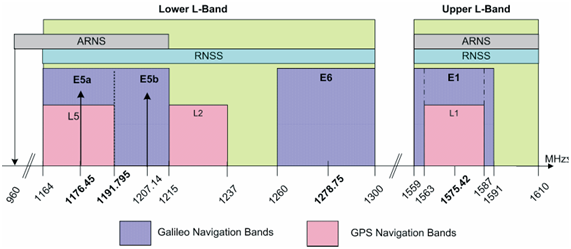
\includegraphics{img/GalileoFrequencyPlan.png}
\caption{Galileo Frequency Plan, Source:\cite{galileoSisIcd}}
\label{fig:galileofrequencyplan}
\end{figure}

Figure \ref{fig:galileofrequencyplan} presents the frequencies used by GPS and Galileo. Using multiple frequencies allows phase measurements without ionosphere errors\cite{instantPPP}. The Galileo E6 signal enables instantaneous convergence for PPP-AR\cite{instantPPP}.

The GNSS receiver presented in \cite{instantPPP} uses E1, E5a, E5b and E6 signals received from one Galileo satellite to compute the ionosphere-free pseudorange, ionospheric delay and four carrier phase ambiguities\cite{instantPPP}. The Galileo E5 could also be used, however, its frequency is so close to E5a and E5b signals that its contribution is negligible\cite{instantPPP}.

\begin{table}[h!]
\centering
\begin{tabular}{|c|c|c|}
    \hline
    System & Frequencies & Range (meters) \\
    \hline
    Galileo & E1, E5a, E5b & 0.416 \\
    \hline
    Galileo & E1, E5a, E6 & 0.193 \\
    \hline
    Galileo & E1, E5b, E6 & 0.268 \\
    \hline
    Galileo & L1, L2, L5 & 0.298 \\
    \hline
\end{tabular}
\caption{Precision for three frequency single satellite configurations. Source: \cite{instantPPP}}
\label{table:20}
\end{table}

In table \ref{table:20} we can observe the precision of positioning that can be obtained in \cite{instantPPP} using 3 different frequency signals. The E1-E5a-E6 configuration has the best result and we observe that the frequency spacing is important for positioning performance.